\documentclass{beamer}

\usepackage{cite}
\usepackage{float}
\usepackage{graphicx}
\usepackage[caption=false]{subfig}
  \DeclareGraphicsExtensions{.png}
\usepackage{amsmath}
\usepackage{amsfonts}
\usepackage{url}
\usepackage[edges]{forest}
\usepackage{tikz}
\usetikzlibrary{shapes,shapes.gates.logic.US,arrows,arrows.meta,chains,calc}
\tikzset{
  -|-/.style={
    to path={
      (\tikztostart) -| ($(\tikztostart)!#1!(\tikztotarget)$) |- (\tikztotarget)
      \tikztonodes
    }
  },
  -|-/.default=0.5,
  |-|/.style={
    to path={
      (\tikztostart) |- ($(\tikztostart)!#1!(\tikztotarget)$) -| (\tikztotarget)
      \tikztonodes
    }
  },
  |-|/.default=0.5,
}
\usepackage{tikz-timing}
\usetikztiminglibrary[new={char=Q,reset char=R}]{counters}
\usepackage{bm,times}
\usepackage{pgfgantt}
\usepackage{indentfirst}
\usepackage{array}
\usepackage{setspace}
\usepackage{caption}
\usepackage{rotating}
\usepackage{hyperref}

%\usetheme{Boadilla}
\usetheme{Hannover}
\mode<presentation>
{
  \usetheme{default}   % or try Darmstadt, Madrid, Warsaw, ...
  \usecolortheme{default} % or try albatross, beaver, crane, ...
  \usefonttheme{default}  % or try serif, structurebold, ...
  \setbeamertemplate{navigation symbols}{}
  \setbeamertemplate{caption}[numbered]
}

\title[EFEAH]{An Extensible Framework\\for Evaluation of Arithmetic Hardware}
\subtitle{}
\author[Zifan Wang]{Zifan Wang \texorpdfstring{\\}{} Supervisor: Dr. James Davis}
\institute[]{Imperial College London}
\date{\today}

\begin{document}

\begin{frame}
  \titlepage
\end{frame}

\begin{frame}
  \tableofcontents
\end{frame}

\section{Background}
\subsection{Motivation}
\begin{frame}{Motivation}
  \begin{itemize}
  \item High-radix online arithmetic needs testbench
  \item Digital designers all use their own testbench
  \item Propose an extensible framework
\end{itemize}
\end{frame}

\section{Design \& Implementation}
\subsection{System}
\begin{frame}[shrink]{System Architecture}
  \begin{figure}[H]
    \centering
    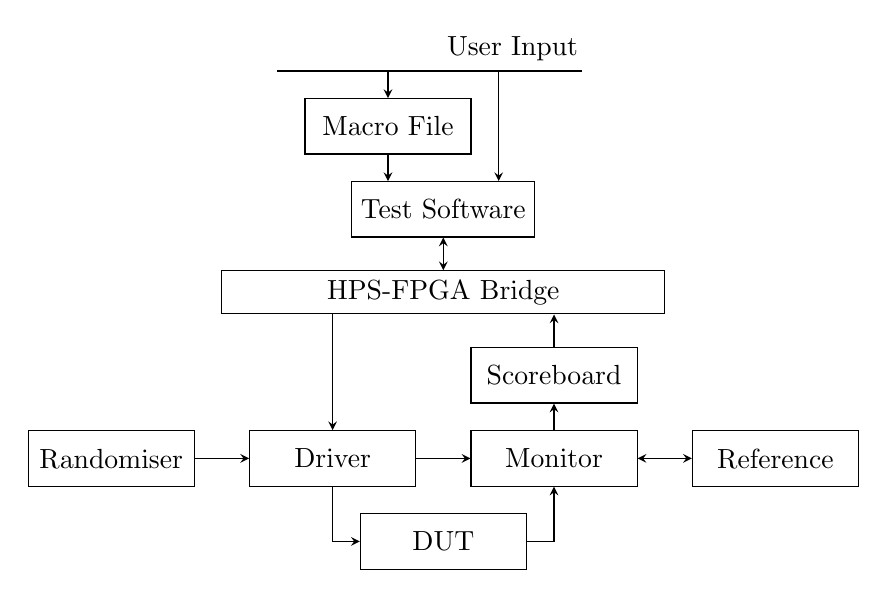
\begin{tikzpicture}
  [
    x=1em, y=1em,
    block/.style =
      {draw, rectangle, align=center, minimum width=6em, minimum height=2em},
    inter/.style =
      {draw, rectangle, align=center, minimum width=16em, minimum height=1em}
  ]
  \node [block] at (-8,3)  (r) {Randomiser};
  \node [block] at ( 0,3)  (d) {Driver};
  \node [block] at ( 4,0)  (t) {DUT};
  \node [block] at ( 8,6)  (s) {Scoreboard};
  \node [block] at ( 8,3)  (m) {Monitor};
  \node [block] at (16,3)  (u) {Reference};
  \node [inter] at ( 4,9)  (b) {HPS-FPGA Bridge};
  \node [block] at ( 4,12) (w) {Test Software};
  \node [block] at ( 2,15) (f) {Macro File};

  \draw[ ->, >=stealth] (r.east)           -- (d.west);
  \draw[ ->, >=stealth] (d.south)          |- (t.west);
  \draw[ ->, >=stealth] (t.east)           -| (m.south);
  \draw[ ->, >=stealth] (m.north)          -- (s.south);
  \draw[ ->, >=stealth] (b.south-|d.north) -- (d.north);
  \draw[ ->, >=stealth] (s.north)          -- (b.south-|s.north);
  \draw[<->, >=stealth] (b.north)          -- (w.south);
  \draw[ ->, >=stealth] (f.south)          -- (w.north-|f.north);
  \draw[ ->, >=stealth] (d.east)           -- (m.west);
  \draw[<->, >=stealth] (m.east)           -- (u.west);
  \draw[ ->, >=stealth] (2, 17)            -- (f.north);
  \draw[ ->, >=stealth] (6, 17)            -- (w.north-|6,17);

  \draw (-2,17) -- ++(6,0) -- node[above] {User Input} ++(5,0);
\end{tikzpicture}
    \label{Block}
  \end{figure}
\end{frame}

\subsection{Hardware}
\begin{frame}[shrink]{Hardware}
  \begin{figure}[H]
    \centering
    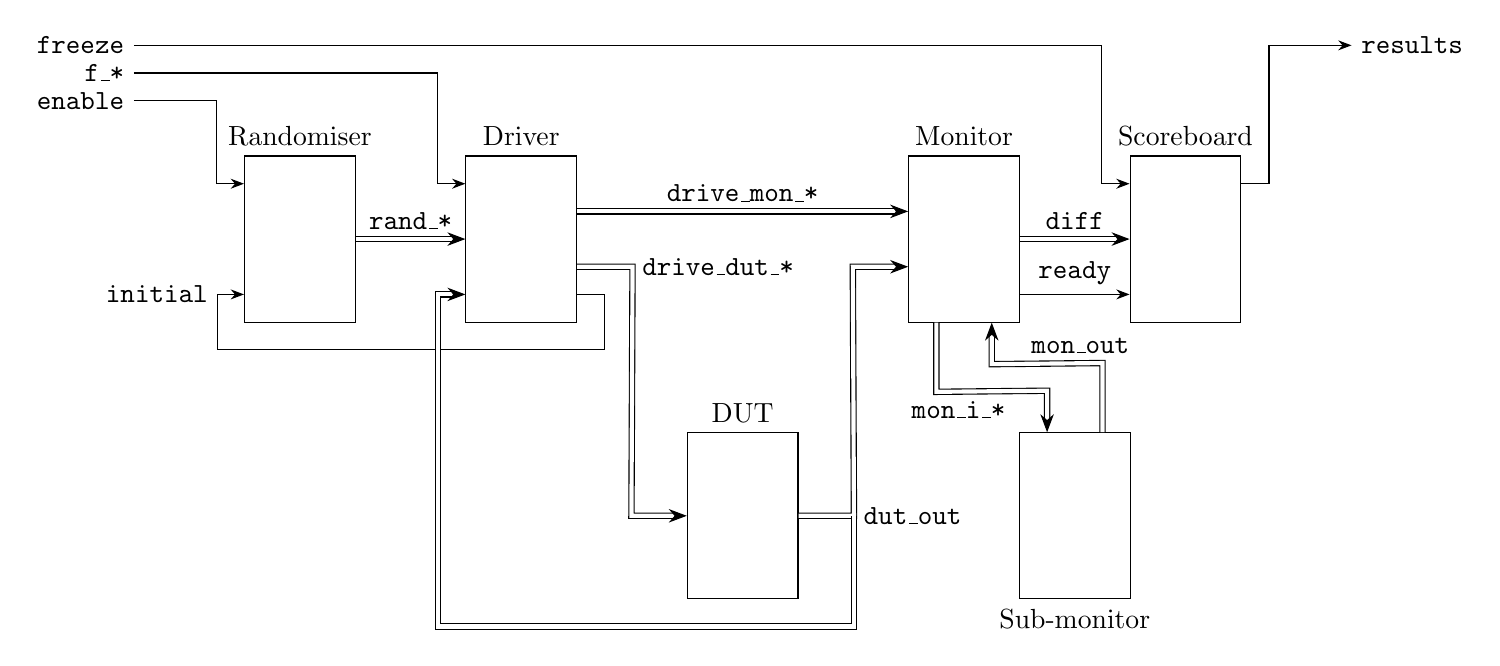
\begin{tikzpicture}
  [
    x=1em, y=1em,
    block/.style =
      {draw, rectangle, align=center, minimum width=4em, minimum height=6em},
    sarrow/.style =
      {>={Stealth}, font=\ttfamily},
    darrow/.style =
      {double distance=1.5pt, >={Stealth}, font=\ttfamily}
  ]
  \node [block, label=above:Randomiser]  at ( 8, 10)  (r) {};
  \node [block, label=above:Driver]      at (16, 10)  (d) {};
  \node [block, label=above:DUT]         at (24,  0)  (t) {};
  \node [block, label=above:Monitor]     at (32, 10)  (m) {};
  \node [block, label=below:Sub-monitor] at (36,  0)  (u) {};
  \node [block, label=above:Scoreboard]  at (40, 10)  (s) {};

  \draw [->, sarrow] (2,15) node[left] {enable}
                      -| ($(r.west)+(-1,2)$)
                      -- ($(r.west)+(0,2)$);
  \draw [->, sarrow] (2,16) node[left] {f\_*}
                      -| ($(d.west)+(-1,2)$)
                      -- ($(d.west)+(0,2)$);
  \draw [->, sarrow] (2,17) node[left] {freeze}
                      -| ($(s.west)+(-1,2)$)
                      -- ($(s.west)+(0,2)$);

  \draw [->, sarrow] ($(d.east)-(0,2)$)
                      -| ++(1,-2)
                      -- ++(-14,0)
                      |- node[left] {initial} ($(r.west)-(0,2)$);
  \draw [->, darrow] ($(r.east)+(0,0)$)
                      -- node[above] {rand\_*} ($(d.west)+(0,0)$);
  \draw [->, darrow] ($(d.east)+(0,1)$)
                      -- node[above] {drive\_mon\_*} ($(m.west)+(0,1)$);
  \draw [->, darrow] ($(d.east)-(0,1)$)
                      -- ++(2,0)
                      -- node[right,pos=0] {drive\_dut\_*} ($(t.west)+(-2,0)$)
                      -- ($(t.west)+(0,0)$);
  \draw [->, darrow] ($(t.east)-(0,0)$)
                      -- ++(2,0)
                      -- node[right,pos=0] {dut\_out} ($(m.west)-(2,1)$)
                      -- ($(m.west)-(0,1)$);
  \draw [->, darrow] ($(t.east)+(2,0)$)
                      |- ($(d.west)-(1,14)$)
                      |- ($(d.west)-(0,2)$);
  \draw [->, darrow] ($(m.south)-(1,0)$)
                      -- ++(0,-2.5)
                      -- node[below,pos=0.2] {mon\_i\_*} ($(u.north)-(1,-1.5)$)
                      -- ($(u.north)-(1,0)$);
  \draw [<-, darrow] ($(m.south)+(1,0)$)
                      -- ++(0,-1.5)
                      -- node[above,pos=0.8] {mon\_out} ($(u.north)+(1,2.5)$)
                      -- ($(u.north)+(1,0)$);
  \draw [->, darrow] ($(m.east)+(0,0)$)
                      -- node[above] {diff} ($(s.west)+(0,0)$);
  \draw [->, sarrow] ($(m.east)-(0,2)$)
                      -- node[above] {ready} ($(s.west)-(0,2)$);
  \draw [->, sarrow] ($(s.east)+(0,2)$)
                      -| ++(1,5)
                      -- (46,17) node[right] {results};

\end{tikzpicture}
    \label{DBlock}
  \end{figure}
\end{frame}

\subsection{Software}
\begin{frame}{Software}
\begin{itemize}
  \item 
\end{itemize}
\end{frame}

\section{Results}
\subsection{Results}
\begin{frame}{Results}
\begin{itemize}
  \item 
\end{itemize}
\end{frame}

\section{Evaluation}
\subsection{Evaluation}
\begin{frame}{Evaluation}
\begin{itemize}
  \item 
\end{itemize}
\end{frame}

\section{Summary}
\begin{frame}{Thank you}
Questions?
\end{frame}

\end{document}